\documentclass{../tex/report}
\usepackage{setspace} % Setting line spacing
\usepackage{ulem} % Underline
\usepackage{caption} % Captioning figures
\usepackage{subcaption} % Subfigures
\usepackage{geometry} % Page layout
\usepackage{multicol} % Columned pages
\usepackage{array,etoolbox}
\usepackage{fancyhdr}
\usepackage{enumitem}
\usepackage[toc,page]{appendix}

% Page layout (margins, size, line spacing)
\geometry{letterpaper, left=1in, right=1in, bottom=1in, top=1in}
\setstretch{1.5}

% Headers
\pagestyle{fancy}
\lhead{PeaPod - Requirements}
\rhead{PeaPod Technologies Inc.}

% Metric counter, referencing commands
\newcounter{metricnumber}
\setcounter{metricnumber}{1}
\newcommand{\metricrow}{M\arabic{metricnumber}}
\newcommand{\mlabel}[1]{\addtocounter{metricnumber}{-1}\refstepcounter{metricnumber}\label{#1}\addtocounter{metricnumber}{1}}
\newcommand{\mref}[1]{\hyperref[#1]{M\ref{#1}}}

\begin{document}

\begin{titlepage}
    \begin{center}
        \vspace*{1.2cm}

        \textbf{\large{PeaPod - Requirements}}

        \vspace{0.5cm}

        Outlining the Requirements for a Design Submission to the \\NASA/CSA Deep Space Food Challenge

        \vfill
        \small{
    \textbf{Jayden Lefebvre - Founder, Lead Engineer}\\
    Port Hope, ON, Canada\\
    \vspace{.5cm}
    \textbf{Nathan Chareunsouk - Design Lead}\\Toronto, ON, Canada\\
    \vspace{.5cm}
    \textbf{Navin Vanderwert - Design Engineer}\\
    BASc Engineering Science (Anticipated 2024), University of Toronto, Toronto, ON, Canada\\
    \vspace{.5cm}
    \textbf{Jonas Marshall - Electronics Engineer}\\
    BASc Computer Engineering (Anticipated 2024), Queen's University, Kingston, ON, Canada\\
    \vspace{.5cm}
    Open-source contributions made by:\\
    \textbf{University of Toronto Agritech}
}

\vspace{1cm}

Primary Contact Email: contact@peapodtech.com
        \vspace{.75cm}

        Revision 0.9\\
        PeaPod Technologies Inc.\\
        July 8th, 2022

    \end{center}
\end{titlepage}

\thispagestyle{plain}

\tableofcontents
\clearpage

\section{Introduction}
\label{sec:intro}

\subsection{Purpose}
\label{sec:purpose}

The purpose of this document is to outline both the \textit{categorical} requirements (Section \ref{sec:requirements}) for a design submission to the NASA/CSA Deep Space Food Challenge (DSFC) \cite{dsfc}, as well as the \textit{scoped} requirements (Section \ref{sec:scope}) for the specific design being proposed by PeaPod Technologies Inc.

The goal of the DSFC is for participants to "Create novel food production technologies or systems that require \uline{minimal inputs} and \uline{maximize safe, nutritious, and palatable food outputs} for \uline{long-duration space missions}, and which have potential to benefit people on Earth." \cite{applicantguide}

\subsection{Framing Structure}
\label{sec:structure}

This document achieves its purpose via "top-down" framing (Section \ref{sec:framing}), with each subsection's entries being derived from the entries of the
previous\footnote{Each objective and metric has a numbered reference to the entry it was derived from (\uline{\textbf{S}}takeholder \uline{\textbf{1}} : S1, \uline{\textbf{H}}igh-\uline{\textbf{L}}evel Objective \uline{\textbf{8}} : HL8, etc.)}.

\begin{itemize}
    \item \textbf{\ref{sec:opportunity} - Opportunity}: A succinct scoped design statement.
    \item \textbf{\ref{sec:requirements} - Challenge Requirements}: Categorical requirements for \textit{any} DSFC submission.
    \item \textbf{\ref{sec:stakeholders} - Stakeholders}: Persons and groups in consideration.
    \item \textbf{\ref{sec:hlos} - High-Level Objectives (HLOs)}: Conceptual aims/"DfX" derived from Requirements and Stakeholders.
    \item \textbf{\ref{sec:llos} - Low-Level Objectives (LLOs)}: Tactical, practical goals derived from HLOs.
    \item \textbf{\ref{sec:metrics} - Metrics}: Granular, quantitative measures of design success, fit, utility, etc. derived from LLOs.
    \item \textbf{\ref{sec:constraints} - Constraints}: \textit{Mandatory} requirements, minimums, and maximums (i.e. true/false, pass/fail) of metrics for the proposed design.
    \item \textbf{\ref{sec:criteria} - Criteria}: \textit{Graded} (i.e. points-based, more/less is better) metrics for the proposed design.
\end{itemize} 

\clearpage
\subsection{Scope and Justification}
\label{sec:scope}

The three underlined criteria in the challenge statement in Section \ref{sec:purpose} have helped to define the scope of the design:
\begin{enumerate}[label=SC\arabic*., ref=SC\arabic*]
    \item \label{sc:1} The longer the duration of the space mission (up to and including interplanetary travel and permanent colonization) the lesser the feasibility of resupply\footnote{Minimal resupply is also listed as a constraint directly in the challenge details \cite{applicantguide,dsfc-phase2}.}. The lesser the feasibility of resupply, and the more minimal the input (i.e. launch mass), the less food will be able to be packed at launch, thus the more the design will need to generate \uline{net-new food grown on-board during the mission}.
    \item \label{sc:2} The minimization of inputs (launch mass), the minimization of other negative criteria such as growth time, design complexity, etc. and the maximization of safety (pathogenic and otherwise) means that the design should focus on \uline{food-producing plant growth}\footnote{This is primarily an issue in-transit; for colonization, non-plant food production systems should definitely be considered.}. Animal food production has been deemed not feasible, and is outside the scope of this design
    \item \label{sc:3} Spacecraft are not good plant growth systems (lack of water access, proper lighting and nutrition, etc.), thus the design should encompass a \uline{plant growth environment} that:
        \begin{enumerate}[label=SC3\alph*., ref=SC3\alph*]
            \item \label{sc:3a} provides of all necessary \uline{plant growth inputs} (water, nutrients, lighting, etc.);
            \item \label{sc:3b} contains or otherwise encompasses a viable \uline{plant growth environment} (temperature, humidity, gas concentrations, airflow, etc.);
            \item \label{sc:3c} has control over all of both a) and b), collectively referred to as the \uline{environment parameters}, producing suitable \uline{environment conditions}.
        \end{enumerate}
    \item \label{sc:4} To maximize safety (of both plants and the crew) and redundancy, and to minimize inputs (required human interaction), the environment should be \uline{automated and isolated} from the spacecraft cabin with regards to all environment conditions (thermal insulation, water-tight, etc.) unless beneficial and efficient (i.e. no loss).
\clearpage
    \item \label{sc:5} A greater degree of nutrition and palatability of food outputs implies a greater variety of plants (incl. leafy greens, fruits, root vegetables, legumes, etc.). As such, the food production system should be able to \uline{generate a continuous and wide variety of environmental conditions} such that virtually \uline{any food plants} could be grown within.
    \item \label{sc:6} The demand for high plant variety, automation, parameter control, efficiency/input minimization (water, nutrients, footprint per plant), etc. implies the use of an \uline{aeroponic plant watering method} \cite{spinoff}.
    \item \label{sc:7} Output nutrient and yield maximization in a controlled-environment implies \uline{environment parameter optimization}. This is best accomplished via data collection of both plant-growth and environment metrics and cross-growth-environment networking (data versatility, sharing, and machine intelligence).
    \item \label{sc:8} A solution focussed on palatability (focus on enjoyable plants) and variety (adaptability to many distinct environment requirements) is not suited to high caloric output. Most plants are simply not capable of producing the required daily caloric output in the space allotted (Section \ref{sec:constraints}). As such, the scope of our solution places \uline{far greater importance on output palatability and variety} (both culinary and nutritional) as well as production of critical micronutrients as opposed to pure caloric yield\footnote{The solution "need not meet the full nutritional requirements of future crews, but can contribute significantly to, and integrate with, a comprehensive food system." \cite{applicantguide}}.
\end{enumerate}

DSFC Phase 1 and 2 development, testing, and assessment is scoped to "Earth-like" operating conditions \cite{applicantguide,dsfc-phase2}:
\begin{itemize}
    \item Gravity (9.81 m/s${}^2$);
    \item Ambient atmospheric pressure (101,325 Pa);
    \item Ambient atmospheric temperature (22 °C);
    \item Ambient atmospheric humidity (50 \%RH);
\end{itemize}

\clearpage
\subsection{Definitions}
\label{sec:definitions}

A number of useful definitions have emerged from the above scoping:
\begin{enumerate}
    \item \textbf{(Plant Growth) Environment} - The holistic environment with which the plant interacts over the course of its growth.
    \item \textbf{(Plant Growth) Environment Parameters} - The independent quantitative parameters defining the Environment (i.e. air temperature, CO${}_2$ concentration).
    \item \textbf{(Plant Growth) Environment Conditions} - The collection of Environment Parameter values at any given time, or, the environment as experienced by the plant.
    \item \textbf{(Plant) Growth System} - Includes the physical enclosure isolating the plant and Environment from the surroundings, as well as any infrastructure required to control the Environment Parameters and generate the Environment by maintaining Environment Conditions. Satisfies all requirements in this document.
    \item \textbf{(Plant) Growth Metrics} - The quantitative measures of plant growth, including yield mass, growth rate, compound concentrations (i.e. nutrients, flavour compounds), caloric density, etc.
    \item \textbf{(Environment) Schedule} - An instruction set outlining the ideal values for each Environment Parameter to be enacted by the Plant Growth System over the course of a growth cycle.
\end{enumerate}

\clearpage
\section{Framing}
\label{sec:framing}

\subsection{Opportunity}
\label{sec:opportunity}

Design an automated and isolated aeroponic plant growth system for the Deep Space Food Challenge \cite{dsfc}, able to generate any environment conditions from a combination of independent environment parameters, with both environment and plant growth metric data collection.

\subsection{Challenge Requirements}
\label{sec:requirements}

The following are the overall challenge requirements compiled from DSFC Applicant Guide details \cite{applicantguide}, the DSFC Phase 2 Instructions \cite{dsfc-phase2}, and an excerpt from NASA-STD-3001: Section 7.1 Food and Nutrition \cite{nutrition}.

\begin{enumerate}[label=R\arabic*., ref=R\arabic*]
    \item \label{r:1} \textbf{Must} help fill food gaps for a \textit{three-year} round-trip mission with \textit{no resupply}:
    \begin{enumerate}[ref=R1\alph*]
        \item \label{r:1a} \textbf{Should} aim to produce food outputs that fulfill \textbf{all daily nutritional needs} for a crew of \textit{four (4)} people;
        \item \label{r:1b} \textbf{Must} maintain food output \textit{safety} and \textit{nutrition} during \textit{all phases} of the mission;
        \item \label{r:1c} \textbf{Must} output food that is \textit{varied, palatable, and acceptable} to the crew for the \textit{duration} of the mission;
        \item \label{r:1d} \textbf{Must} produce food outputs that require \textit{no additional processing time}\footnote{It is assumed that fresh (or packaged unprepared) edible plant products are already prepared on existing space missions, and that this preparation meets this requirement.};
    \end{enumerate}
    \item \label{r:2} \textbf{Should} improve the accessibility of food on Earth by enhancing local production; in particular, via production directly in urban centres and in remote and harsh environments;
    \item \label{r:3} \textbf{Must} aim to achieve the \textit{greatest food output} with \textit{minimal inputs} and \textit{minimal waste};
    \item \label{r:4} \textbf{Must} transmit \textit{operational data and limited video} to a remote location, and be able to receive periodic \textit{operational commands};
    \item \label{r:5} \textbf{Must} operate under Earth-like conditions (See Section \ref{sec:scope});
\end{enumerate}

\clearpage
\subsection{Stakeholders}
\label{sec:stakeholders}
\setstretch{1} % Change line spacing for the more list-heavy sections

\begin{enumerate}[label=S\arabic*., ref=S\arabic*]
    \item \label{s:1} Crew - Time requirement; output safety, palatability, quality
    \item \label{s:2} NASA/CSA Stakeholders - Feasability; operational safety; input limitation, optimization
\end{enumerate}

\subsection{Objectives}
\label{sec:objectives}

% High-Level
\begin{multicols}{2}[\subsubsection{High-Level}\label{sec:hlos}]
    \begin{enumerate}[label=HL\arabic*., ref=HL\arabic*]
        \item \label{hl:output} Food Output Suitability                                 \hfill (\ref{s:1}, \ref{r:1}, \ref{r:1a}, \ref{r:1c}, \ref{r:1d}, \ref{r:2})
        \item \label{hl:environment} Environment Control, Automation, and Optimization  \hfill (\ref{s:2}, \ref{r:1b}, \ref{r:1d}, \ref{r:2}, \ref{r:3}, \ref{r:4})
        \item \label{hl:outputsafety} Output Safety                                     \hfill (\ref{s:1}, \ref{s:2}, \ref{r:1b}, \ref{r:2})
        \item \label{hl:efficiency} Time and Resource Efficiency                        \hfill (\ref{s:1}, \ref{s:2}, \ref{r:1d}, \ref{r:2}, \ref{r:3})
        \item \label{hl:safety} Process Safety, Stability, Reliability                  \hfill (\ref{s:1}, \ref{s:2}, \ref{r:1b})
        \item \label{hl:feasibility} Feasibility                                        \hfill (\ref{s:2}, \ref{r:2}, \ref{r:5})
    \end{enumerate}
\end{multicols}

% Low-Level
\begin{multicols}{2}[\subsubsection{Low-Level}\label{sec:llos}]
    \begin{enumerate}[label=LL\arabic*., ref=LL\arabic*]
        \item \label{ll:output_variety} Output Food Variety                     \hfill (\ref{hl:output})
        \item \label{ll:output_palatability} Output Food Palatability           \hfill (\ref{hl:output})
        \item \label{ll:output_nutrients} Nutrient Output                       \hfill (\ref{hl:output}, \ref{hl:efficiency})
        \item \label{ll:output_energy} Caloric Output                           \hfill (\ref{hl:output}, \ref{hl:efficiency})
        \item \label{ll:control_airtemp} Leaf-Zone Thermoregulation             \hfill (\ref{hl:environment}, \ref{hl:efficiency})
        \item \label{ll:control_airhum} Leaf-Zone Humidity Control              \hfill (\ref{hl:environment})
        \item \label{ll:control_gas} Gas Concentration Control                  \hfill (\ref{hl:environment})
        \item \label{ll:control_light} Lighting Control                         \hfill (\ref{hl:environment}, \ref{hl:efficiency})
        \item \label{ll:insulateisolate} Insulation, Isolation                  \hfill (\ref{hl:environment}, \ref{hl:outputsafety}, \ref{hl:efficiency})
        \item \label{ll:control_aircirculation} Air Circulation Control         \hfill (\ref{hl:environment}, \ref{hl:outputsafety})
        \item \label{ll:control_nutrientsolution} Nutrient Solution Control     \hfill (\ref{hl:environment})
        \item \label{ll:control_roottemp} Root-Zone Thermoregulation            \hfill (\ref{hl:environment})
        \item \label{ll:germinationsuccess} Germination Success                 \hfill (\ref{hl:environment}, \ref{hl:efficiency}, \ref{hl:safety})
        \item \label{ll:automation} High Degree of Automation                   \hfill (\ref{hl:outputsafety}, \ref{hl:efficiency})
        \item \label{ll:efficiency_energy} Energy Efficiency                    \hfill (\ref{hl:efficiency})
        \item \label{ll:efficiency_water} Water Usage                           \hfill (\ref{hl:efficiency})
        \item \label{ll:time_germination} Germination Time                      \hfill (\ref{hl:efficiency})
        \item \label{ll:time_growth} Growth Time                                \hfill (\ref{hl:efficiency})
        \item \label{ll:time_harvest} Time-To-Harvest/-Reharvest                \hfill (\ref{hl:efficiency})
        \item \label{ll:crosscontamination} Potential for Cross-Contamination   \hfill (\ref{hl:outputsafety})
        \item \label{ll:safety_process} Environmental, Process Safety           \hfill (\ref{hl:safety})
        \item \label{ll:output_safety} Output Consumption Safety                \hfill (\ref{hl:output}, \ref{hl:safety})
        \item \label{ll:reliability} Reliability                                \hfill (\ref{hl:safety})
        \item \label{ll:stability_input} Input Stability                        \hfill (\ref{hl:safety})
        \item \label{ll:stability_output} Output Shelf Life                     \hfill (\ref{hl:safety})
        \item \label{ll:cost} Cost                                              \hfill (\ref{hl:feasibility})
        \item \label{ll:size} Size                                              \hfill (\ref{hl:feasibility})
    \end{enumerate}
\end{multicols}

\clearpage
\subsection{Metrics}
\label{sec:metrics}

\begin{tabular}{| @{\makebox[2.4em][c]{\metricrow}} | p{8.7cm} | p{5.9cm} |} 
    \hline
    \multicolumn{1}{| @{\makebox[2.4em][c]{\textbf{\#}}} | l |}
    {\textbf{Metric}}                                                                                                           & \textbf{Units}                                        \\ \hline
    Plant Species Capability                    \mlabel{m:plant_variety}            \hfill (\ref{ll:output_variety})            & Y/N (per plant species)                               \\ \hline
    Palatability of Output                      \mlabel{m:palatability}             \hfill (\ref{ll:output_palatability})       & 1-9 Hedonic (per plant)                               \\ \hline
    Protein Output                              \mlabel{m:nutrient_protein}         \hfill (\ref{ll:output_nutrients})          & g/kg body mass/crewmember/day                         \\ \hline
    Protein Output Calories                     \mlabel{m:nutrient_proteincal}      \hfill (\ref{ll:output_nutrients})          & kCal/day/crewmember (\%TDEI)                          \\ \hline
    Carbohydrate Output Calories                \mlabel{m:nutrient_carbs}           \hfill (\ref{ll:output_nutrients})          & kCal/day/crewmember (\%TDEI)                          \\ \hline
    Lipid Output Calories                       \mlabel{m:nutrient_fats}            \hfill (\ref{ll:output_nutrients})          & kCal/day/crewmember (\%TDEI)                          \\ \hline
    $\Omega$-6 Fatty Acid Output                \mlabel{m:nutrient_om6fats}         \hfill (\ref{ll:output_nutrients})          & g/day/crewmember                                      \\ \hline
    $\Omega$-3 Fatty Acid Output                \mlabel{m:nutrient_om3fats}         \hfill (\ref{ll:output_nutrients})          & g/day/crewmember                                      \\ \hline
    Saturated Fat Output Calories               \mlabel{m:nutrient_satfats}         \hfill (\ref{ll:output_nutrients})          & kCal/day/crewmember (\%TDEI)                          \\ \hline
    Trans Fatty Acids Output                    \mlabel{m:nutrient_transfats}       \hfill (\ref{ll:output_nutrients})          & kCal/crewmember (\%TDEI)                              \\ \hline
    Cholesterol Output                          \mlabel{m:nutrient_cholesterol}     \hfill (\ref{ll:output_nutrients})          & mg/day/crewmember                                     \\ \hline
    Fiber Output                                \mlabel{m:nutrient_fiber}           \hfill (\ref{ll:output_nutrients})          & g/day/crewmember                                      \\ \hline
    Caloric Output                              \mlabel{m:output_calories}          \hfill (\ref{ll:output_energy})             & kCal/day/crewmember                                   \\ \hline
    Air Temperature Control Range               \mlabel{m:airtemp_range}            \hfill (\ref{ll:control_airtemp})           & min, max °C                                           \\ \hline
    Air Temperature Control Rate                \mlabel{m:airtemp_rate}             \hfill (\ref{ll:control_airtemp})           & $\Delta$°C/sec at each °C                             \\ \hline
    Air Temperature Control Stability           \mlabel{m:airtemp_stability}        \hfill (\ref{ll:control_airtemp})           & $\pm$°C at each °C                                    \\ \hline
    Air Humidity Control Range                  \mlabel{m:airhum_range}             \hfill (\ref{ll:control_airhum})            & min, max \%RH                                         \\ \hline
    Air Humidity Control Rate                   \mlabel{m:airhum_rate}              \hfill (\ref{ll:control_airhum})            & $\Delta$\%RH/sec at each \%RH                         \\ \hline
    Air Humidity Control Stability              \mlabel{m:airhum_stability}         \hfill (\ref{ll:control_airhum})            & $\pm$\%RH at each \%RH                                \\ \hline
    CO${}_2$ Supplementation Range              \mlabel{m:co2_range}                \hfill (\ref{ll:control_gas})               & max ppm CO${}_2$                                      \\ \hline
    CO${}_2$ Concentration Control Rate         \mlabel{m:co2_rate}                 \hfill (\ref{ll:control_gas})               & ppm CO${}_2$/sec at each ppm CO${}_2$                 \\ \hline
    CO${}_2$ Concentration Control Stability    \mlabel{m:co2_stability}            \hfill (\ref{ll:control_gas})               & $\pm$ppm CO${}_2$ at each ppm CO${}_2$                \\ \hline
    Light Spectrum Wavelength Range             \mlabel{m:light_waverange}          \hfill (\ref{ll:control_light})             & min, max nm                                           \\ \hline
    Light Spectrum PAR Match                    \mlabel{m:light_parmatch}           \hfill (\ref{ll:control_light})             & \% (each plant)                                       \\ \hline
    Light Intensity Control Range               \mlabel{m:lightintensity_range}     \hfill (\ref{ll:control_light})             & min, max $\mu$mol m${}^{-2}$sec${}^{-1}$ at each nm   \\ \hline
    Light Intensity Control Stability           \mlabel{m:lightintensity_stability} \hfill (\ref{ll:control_light})             & $\pm\mu$mol m${}^{-2}$sec${}^{-1}$ at each nm         \\ \hline
    Light Loss, Capture by Surfaces             \mlabel{m:light_loss}               \hfill (\ref{ll:insulateisolate})           & \%                                                    \\ \hline
    Outside Light Penetration                   \mlabel{m:light_isolation}          \hfill (\ref{ll:insulateisolate})           & \%                                                    \\ \hline
    Heat Loss                                   \mlabel{m:heat_loss}                \hfill (\ref{ll:insulateisolate})           & $\pm$W at each °C                                     \\ \hline
    Water Loss due to Leaks, Evaporation        \mlabel{m:water_loss}               \hfill (\ref{ll:insulateisolate})           & mL/hr                                                 \\ \hline
    Internal Circulation Airflow Control Range  \mlabel{m:circulation_range}        \hfill (\ref{ll:control_aircirculation})    & min, max m${}^3$/min                                  \\ \hline
    Gas Exchange due to Leaks                   \mlabel{m:gas_loss}                 \hfill (\ref{ll:control_aircirculation})    & m${}^3$/min                                           \\ \hline
    Maximum Intentional Gas Exchange            \mlabel{m:gas_maxrate}              \hfill (\ref{ll:control_aircirculation})    & m${}^3$/min                                           \\ \hline
    Nutrient Sol'n Delivery Control Range       \mlabel{m:solutionrate_range}       \hfill (\ref{ll:control_nutrientsolution})  & min, max mL/sec                                       \\ \hline
    Nutrient Sol'n Delivery Control Rate        \mlabel{m:solutionrate_rate}        \hfill (\ref{ll:control_nutrientsolution})  & $\Delta$mL/sec${}^2$ at each mL/sec                   \\ \hline
    Nutrient Sol'n Delivery Control Stability   \mlabel{m:solutionrate_stability}   \hfill (\ref{ll:control_nutrientsolution})  & $\pm$mL/sec at each mL/sec                            \\ \hline
    Nutrient Concentrations Control Range       \mlabel{m:nutrient_range}           \hfill (\ref{ll:control_nutrientsolution})  & min, max ppm (each nutrient)                          \\ \hline
    Nutrient Concentrations Control Rate        \mlabel{m:nutrient_rate}            \hfill (\ref{ll:control_nutrientsolution})  & $\Delta$ppm/sec at each ppm (each nutr.)              \\ \hline
    Nutrient Concentrations Control Stability   \mlabel{m:nutrient_stability}       \hfill (\ref{ll:control_nutrientsolution})  & $\pm$ppm at each ppm (each nutrient)                  \\ \hline
\end{tabular}
\clearpage

\textbf{\large{2.5 \ \ Metrics (Cont'd)}}
\normalsize

\begin{tabular}{| @{\makebox[2.4em][c]{\metricrow}} | p{9.45cm} | p{5.1cm} |} 
    \hline
    \multicolumn{1}{| @{\makebox[2.4em][c]{\textbf{\#}}} | l |}
    {\textbf{Metric}}                                                                                                           & \textbf{Units}        \\ \hline
    Nutrient Sol'n Temp. Control Range          \mlabel{m:solutiontemp_range}           \hfill (\ref{ll:control_roottemp})      & min, max °C           \\ \hline
    Nutrient Sol'n Temp. Control Rate           \mlabel{m:solutiontemp_rate}            \hfill (\ref{ll:control_roottemp})      & °C/sec at each °C     \\ \hline
    Nutrient Sol'n Temp Control Stability       \mlabel{m:solutiontemp_stability}       \hfill (\ref{ll:control_roottemp})      & $\pm$°C at each °C    \\ \hline
    Germination Success Rate                    \mlabel{m:germinationsuccess}           \hfill (\ref{ll:germinationsuccess})    & \%                    \\ \hline
    Time Requirement - Maintenance              \mlabel{m:time_maintenance}             \hfill (\ref{ll:automation})            & hrs/week              \\ \hline
    Time Requirement - Setup                    \mlabel{m:time_setup}                   \hfill (\ref{ll:automation})            & hrs                   \\ \hline
    Energy Efficiency - Power vs. kCal          \mlabel{m:efficiency_energy}            \hfill (\ref{ll:efficiency_energy})     & \%                    \\ \hline
    Necessary Water Waste per Day               \mlabel{m:efficiency_water}             \hfill (\ref{ll:efficiency_water})      & L/day                 \\ \hline
    Initial Water Requirement                   \mlabel{m:water_initial}                \hfill (\ref{ll:efficiency_water})      & L                     \\ \hline
    Reharvest Period - Fruiting Plants          \mlabel{m:time_reharvest}               \hfill (\ref{ll:time_harvest})          & days (each plant)     \\ \hline
    Germination Time                            \mlabel{m:time_germination}             \hfill (\ref{ll:time_germination})      & days (each plant)     \\ \hline
    Time to Harvest                             \mlabel{m:time_harvest}                 \hfill (\ref{ll:time_growth})           & days (each plant)     \\ \hline
    Potential for Contamination - Germination   \mlabel{m:contamination_germination}    \hfill (\ref{ll:crosscontamination})    & \% (each event)       \\ \hline 
    Potential for Contamination - Planting      \mlabel{m:contamination_planting}       \hfill (\ref{ll:crosscontamination})    & \% (each event)       \\ \hline
    Potential for Contamination - Harvest       \mlabel{m:contamination_harvest}        \hfill (\ref{ll:crosscontamination})    & \% (each event)       \\ \hline
    Use of Hazardous Compounds                  \mlabel{m:hazards_compounds}            \hfill (\ref{ll:safety_process})        & Y/N                   \\ \hline
    Cleaning Hazards                            \mlabel{m:hazards_cleaning}             \hfill (\ref{ll:safety_process})        & Y/N                   \\ \hline
    Physical, Chemical, Bio Hazards             \mlabel{m:hazards_other}                \hfill (\ref{ll:safety_process})        & Y/N                   \\ \hline
    Consumption Safety                          \mlabel{m:safety_consumption}           \hfill (\ref{ll:output_safety})         & \%                    \\ \hline
    Loss of Functionality Over 3 Years          \mlabel{m:longevity}                    \hfill (\ref{ll:reliability})           & \%                    \\ \hline
    Input Lifetime while Safe, Useful           \mlabel{m:shelflife_input}              \hfill (\ref{ll:stability_input})       & Days                  \\ \hline
    Output Shelf Life while Safe, Quality       \mlabel{m:shelflife_output}             \hfill (\ref{ll:stability_output})      & Days                  \\ \hline
    Cost                                        \mlabel{m:cost}                         \hfill (\ref{ll:cost})                  & CAD                   \\ \hline
    Outer Dimensions                            \mlabel{m:dimensions}                   \hfill (\ref{ll:size})                  & m (W, D, H)           \\ \hline
    Outer Volume                                \mlabel{m:volume}                       \hfill (\ref{ll:size})                  & m${}^3$               \\ \hline
    Power Consumption                           \mlabel{m:power}                        \hfill (\ref{ll:size})                  & W                     \\ \hline
    Mass                                        \mlabel{m:mass}                         \hfill (\ref{ll:size})                  & kg                    \\ \hline
\end{tabular}

\subsection{Constraints}
\label{sec:constraints}

\begin{tabular}{|l|p{14.35cm}|}
    \hline
    \textbf{Metric}                 & \textbf{Constraint                                                \hfill Justification}                                   \\ \hline
    \mref{m:palatability}           & $\ge$ 6.0/9.0 Hedonic                                             \hfill \cite{applicantguide,dsfc-phase2}                \\ \hline
    \mref{m:nutrient_protein}       & $\approx$ 0.27g                                                   \hfill \cite{applicantguide,dsfc-phase2,nutrition}      \\ \hline
    \mref{m:nutrient_proteincal}    & $\le$11.67\% TDEI                                                 \hfill \cite{applicantguide,dsfc-phase2,nutrition}      \\ \hline
    \mref{m:nutrient_carbs}         & 50-55\% TDEI                                                      \hfill \cite{applicantguide,dsfc-phase2,nutrition}      \\ \hline
    \mref{m:nutrient_fats}          & 25-35\% TDEI                                                      \hfill \cite{applicantguide,dsfc-phase2,nutrition}      \\ \hline
    \mref{m:nutrient_om6fats}       & $\approx$14g                                                      \hfill \cite{applicantguide,dsfc-phase2,nutrition}      \\ \hline
    \mref{m:nutrient_om3fats}       & 1.1-1.6g                                                          \hfill \cite{applicantguide,dsfc-phase2,nutrition}      \\ \hline
    \mref{m:nutrient_satfats}       & <7\% TDEI                                                         \hfill \cite{applicantguide,dsfc-phase2,nutrition}      \\ \hline
    \mref{m:nutrient_transfats}     & <1\% TDEI                                                         \hfill \cite{applicantguide,dsfc-phase2,nutrition}      \\ \hline
    \mref{m:nutrient_cholesterol}   & <300mg                                                            \hfill \cite{applicantguide,dsfc-phase2,nutrition}      \\ \hline
    \mref{m:nutrient_fiber}         & 21-38g                                                            \hfill \cite{applicantguide,dsfc-phase2,nutrition}      \\ \hline
    \mref{m:airtemp_range}          & Min < 15°C, Max > 30°C                                            \hfill (\ref{sc:5})                                     \\ \hline % TODO: Source?
    \mref{m:airhum_range}           & Min < 20 \%RH, Max > 90 \%RH                                      \hfill (\ref{sc:5})                                     \\ \hline % TODO: Source?
    \mref{m:co2_range}              & >1000ppm ($\approx$600 above ambient)                             \hfill (\ref{sc:5})                                     \\ \hline
    \mref{m:light_waverange}        & Min < 300nm\footnotemark[6] (UV), Max > 800nm (IR)                \hfill (\ref{sc:5}, \ref{sc:7}) \cite{uvc-disinfection} \\ \hline % TODO: Source? Disinfection?
    \mref{m:light_parmatch}         & $\ge$ 95\% match                                                  \hfill (\ref{sc:5})                                     \\ \hline % TODO: Source?
    \mref{m:lightintensity_range}   & Min = 0, Max $\ge$ typical horticulture                           \hfill (\ref{sc:5}, \ref{sc:7})                         \\ \hline % TODO: Source?
    \mref{m:circulation_range}      & Min = 0 m${}^3$/min, Max $\ge$ 2 m${}^3$/min                      \hfill (\ref{sc:5}, \ref{sc:7})                         \\ \hline
    \mref{m:solutionrate_range}     & Min = 0, Max $\ge$ max plant requirement                          \hfill (\ref{sc:5}, \ref{sc:7})                         \\ \hline % TODO: Source?
    \mref{m:solutiontemp_range}     & Min < 10°C, Max > 25°C                                            \hfill (\ref{sc:5})                                     \\ \hline % TODO: Source?
    \mref{m:nutrient_range}         & Min = 0, Max $\ge$ max plant requirement                          \hfill (\ref{sc:5}, \ref{sc:7})                         \\ \hline % TODO: Source?
    \mref{m:time_maintenance}       & 0.5 hrs/week                                                      \hfill \cite{dsfc-phase2}                               \\ \hline
    \mref{m:efficiency_water}       & $\le$4L/day                                                       \hfill \cite{dsfc-phase2}                               \\ \hline
    \mref{m:water_initial}          & $\le$80L                                                          \hfill \cite{dsfc-phase2}                               \\ \hline
    \mref{m:longevity}              & $\le$10\%                                                         \hfill \cite{applicantguide,dsfc-phase2}                \\ \hline
    \mref{m:shelflife_input}        & $\ge$3 years (1095 days)                                          \hfill \cite{applicantguide,dsfc-phase2}                \\ \hline
    \mref{m:shelflife_output}       & $\ge$3 days                                                       \hfill \cite{dsfc-phase2}                               \\ \hline
    \mref{m:dimensions}             & Fits through 1.07m x 1.90m doorway; W<1.829m, D<2.438m, H<2.591m  \hfill \cite{applicantguide,dsfc-phase2}                \\ \hline
    \mref{m:volume}                 & $\le$ 2 m${}^3$                                                   \hfill \cite{applicantguide,dsfc-phase2}                \\ \hline
    \mref{m:power}                  & Avg. <1500W; Peak < 3000W                                         \hfill \cite{applicantguide,dsfc-phase2}                \\ \hline
\end{tabular}
\vfill
\footnotetext[6]{Also for disinfection purposes.}

\subsection{Criteria}
\label{sec:criteria}

\begin{tabular}{|l|p{14.35cm}|}
    \hline
    \textbf{Metric}                     & \textbf{Criteria          \hfill Justification}                       \\ \hline
    \mref{m:plant_variety}              & Should Maximize           \hfill (\ref{r:1c}, \ref{r:3})              \\ \hline
    \mref{m:output_calories}            & Should Maximize           \hfill (\ref{r:1}, \ref{r:1a}, \ref{r:3})   \\ \hline
    \mref{m:airtemp_rate}               & Should Maximize           \hfill (\ref{sc:5}, \ref{sc:7})             \\ \hline
    \mref{m:airtemp_stability}          & Should Minimize           \hfill (\ref{sc:5}, \ref{sc:7})             \\ \hline
    \mref{m:airhum_rate}                & Should Maximize           \hfill (\ref{sc:5}, \ref{sc:7})             \\ \hline
    \mref{m:airhum_stability}           & Should Minimize           \hfill (\ref{sc:5}, \ref{sc:7})             \\ \hline
    \mref{m:co2_rate}                   & Should Maximize           \hfill (\ref{sc:5}, \ref{sc:7})             \\ \hline
    \mref{m:co2_stability}              & Should Minimize           \hfill (\ref{sc:5}, \ref{sc:7})             \\ \hline
    \mref{m:lightintensity_stability}   & Should Minimize           \hfill (\ref{sc:5}, \ref{sc:7})             \\ \hline
    \mref{m:light_loss}                 & Should Minimize           \hfill (\ref{r:3})                          \\ \hline
    \mref{m:light_isolation}            & Should Minimize           \hfill (\ref{sc:5})                         \\ \hline
    \mref{m:heat_loss}                  & Should Minimize           \hfill (\ref{r:3})                          \\ \hline
    \mref{m:water_loss}                 & Should Minimize           \hfill (\ref{r:1b})                         \\ \hline
    \mref{m:gas_loss}                   & Should Minimize           \hfill (\ref{r:3})                          \\ \hline
    \mref{m:gas_maxrate}                & Should Maximize           \hfill (\ref{sc:5}, \ref{sc:7})             \\ \hline
    \mref{m:solutionrate_rate}          & Should Maximize           \hfill (\ref{sc:5}, \ref{sc:7})             \\ \hline
    \mref{m:solutionrate_stability}     & Should Minimize           \hfill (\ref{sc:5}, \ref{sc:7})             \\ \hline
    \mref{m:solutiontemp_rate}          & Should Maximize           \hfill (\ref{sc:5}, \ref{sc:7})             \\ \hline
    \mref{m:solutiontemp_stability}     & Should Minimize           \hfill (\ref{sc:5}, \ref{sc:7})             \\ \hline
    \mref{m:nutrient_rate}              & Should Maximize           \hfill (\ref{sc:5}, \ref{sc:7})             \\ \hline
    \mref{m:nutrient_stability}         & Should Minimize           \hfill (\ref{sc:5}, \ref{sc:7})             \\ \hline
    \mref{m:germinationsuccess}         & Should Maximize           \hfill (\ref{r:1}, \ref{r:1b})              \\ \hline
    \mref{m:time_setup}                 & Should Minimize           \hfill (\ref{s:1})                          \\ \hline
    \mref{m:efficiency_energy}          & Should Maximize           \hfill (\ref{r:3})                          \\ \hline
    \mref{m:time_reharvest}             & Should Minimize           \hfill (\ref{r:1b}, \ref{r:3})              \\ \hline
    \mref{m:time_germination}           & Should Minimize           \hfill (\ref{r:1b})                         \\ \hline
    \mref{m:time_harvest}               & Should Minimize           \hfill (\ref{r:1b})                         \\ \hline
    \mref{m:contamination_germination}  & Should Minimize           \hfill (\ref{r:1b})                         \\ \hline
    \mref{m:contamination_planting}     & Should Minimize           \hfill (\ref{r:1b})                         \\ \hline
    \mref{m:contamination_harvest}      & Should Minimize           \hfill (\ref{r:1b})                         \\ \hline
    \mref{m:hazards_compounds}          & Should Avoid, Mitigate    \hfill (\ref{r:1b})                         \\ \hline
    \mref{m:hazards_cleaning}           & Should Avoid, Mitigate    \hfill (\ref{r:1b})                         \\ \hline
    \mref{m:hazards_other}              & Should Avoid, Mitigate    \hfill (\ref{r:1b})                         \\ \hline
    \mref{m:safety_consumption}         & Should Avoid, Mitigate    \hfill (\ref{r:1b})                         \\ \hline
    \mref{m:cost}                       & Could Minimize            \hfill (\ref{s:2})                          \\ \hline
    \mref{m:mass}                       & Should Minimize           \hfill (\ref{r:3})                          \\ \hline
\end{tabular}

% Refer to Appendix \ref{sec:assessment} for prototype verification Assessment Criteria (categories, weights, etc.).

\clearpage

\section{Reference Designs}

\subsection{Open Agriculture Initiative - Personal Food Computer}

% Project Homepage: https://www.media.mit.edu/groups/open-agriculture-openag/overview/
% Design Repositories: https://github.com/OpenAgricultureFoundation
% PFC White Paper: PDF in Discord
    % Citation: \cite{mit-openag}
% OpenAG White Paper: PDF in Discord
    % Citation: \cite{mit-pfc}

% Half-decent summary: https://www.notion.so/Open-Agriculture-Initiative-OpenAG-cfa5031e2b244093a37158fe1a99ec12

\subsubsection{Overview}

The Open Agriculture Initiative (OpenAG) was a project launched by the MIT Media Lab with the goal to "Build open resources to enable a global community to accelerate digital agricultural innovation" \cite{mit-openag}.

One of their primary developments was an open-source controlled-environment agriculture micro-greenhouse, the Personal Food Computer (PFC) \cite{mit-pfc}. The PFC controls all environmental growing parameters and collects data during the growth cycle.
Data can be collected by users and shared between members of the open-source community. This allows for the creation of reproducible "climate recipes" where other devices with similar abilities can reliably generate the same environment and (ideally) attain the same plant growth results.

\begin{figure}[h]
    \centering
    \begin{subfigure}[b]{0.08\textwidth}
        \hfill
    \end{subfigure}
    \begin{subfigure}[b]{0.40\textwidth}
        \centering
        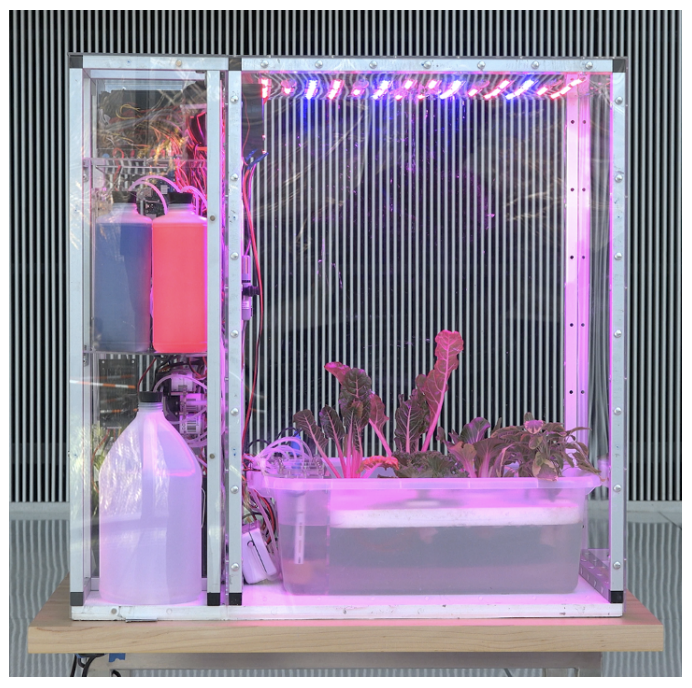
\includegraphics[width=\textwidth]{../assets/pfc-built.png}
        \caption{Assembled PFC v1}
        \label{fig:pfc-built}
    \end{subfigure}
    \hfill
    \begin{subfigure}[b]{0.26\textwidth}
        \centering
        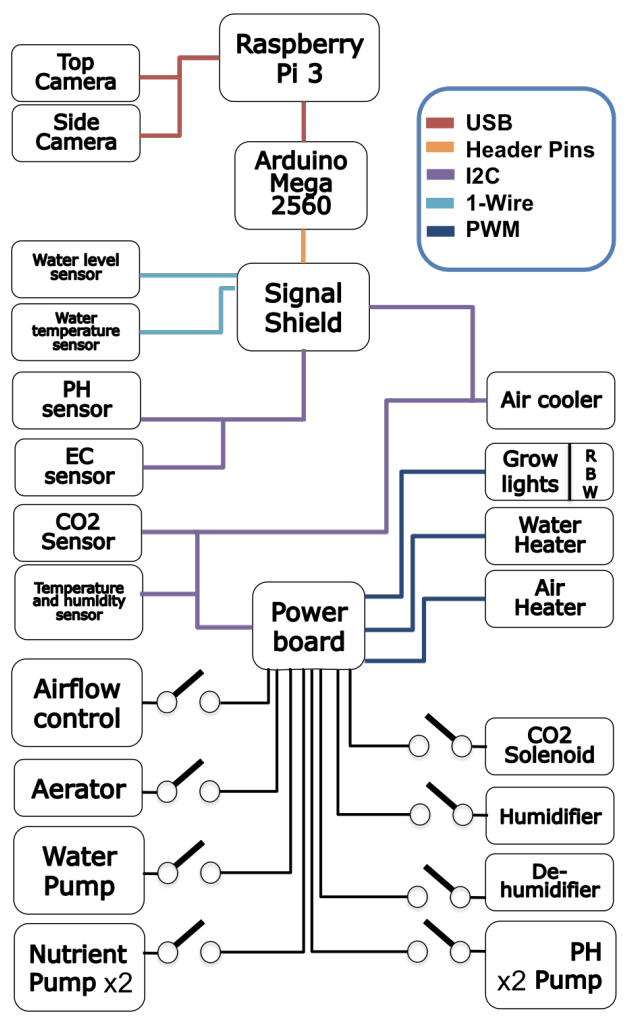
\includegraphics[width=\textwidth]{../assets/pfc-components.png}
        \caption{PFC component diagram}
        \label{fig:pfc-components}
    \end{subfigure}
    \begin{subfigure}[b]{0.10\textwidth}
        \hfill
    \end{subfigure}
    \caption{Personal Food Computer v1 \cite{mit-pfc}}
    \label{fig:pfc}
\end{figure}

\subsubsection{Analysis}

One of the design's major flaws is in its implementation. Despite the claim that the PFC focusses on viable environment generation (Scope \ref{sc:3a}-\ref{sc:3c}) and continuity and range of environment conditions (Scope \ref{sc:5}) \cite{mit-basil}, in practice, it failed to produce food outputs (Requirement \ref{r:1}) \cite{mit-wfp}.
In addition, the PFC utilizes Deep Water Culture (DWC) hydroponics \cite{mit-pfc}, as opposed to aeroponics, resulting in a lowered water efficiency (Objective \ref{ll:efficiency_water}) and decreased control over water conditions (Objective \ref{ll:control_nutrientsolution}).

However, the array of sensors and actuators included in the design (See \ref{fig:pfc-components}), as well as the principle of plant phenomenology optimization \cite{mit-openag}, is informative in meeting Requirement \ref{r:3} and their attempts can serve as a basis for understanding Scope \ref{sc:3} and \ref{sc:5}.

\subsubsection{Assessment}

\textbf{Objectives Considered}: \ref{ll:output_variety}, \ref{ll:output_palatability} (via \ref{sc:5}), \ref{ll:control_airtemp}. \ref{ll:control_airhum}, \ref{ll:control_light}, \ref{ll:control_aircirculation}, \ref{ll:control_nutrientsolution}, \ref{ll:automation}

\textbf{Objectives Not Considered}: \ref{ll:output_energy}, \ref{ll:insulateisolate}, \ref{ll:germinationsuccess}, \ref{ll:efficiency_energy}, \ref{ll:efficiency_water}, \ref{ll:time_germination}, \ref{ll:time_growth}, \ref{ll:time_harvest}, \ref{ll:crosscontamination}

\begin{figure}[h]
    \centering
    \begin{tabular}{|l|l|c|}
        \hline
        \textbf{Metric}                     & \textbf{Value}    & \textbf{Met?}         \\ \hline
        \mref{m:palatability}               & N/A (Presumed Y)  & \cellcolor{red} N     \\ \hline
        \mref{m:airtemp_range}              & N/A (Presumed Y)  & \cellcolor{red} N     \\ \hline % TODO: Source?
        \mref{m:airhum_range}               & N/A (Presumed Y)  & \cellcolor{red} N     \\ \hline % TODO: Source?
        \mref{m:co2_range}                  & N/A (Presumed N)  & \cellcolor{red} N     \\ \hline
        \mref{m:light_waverange}            & 448-710nm         & \cellcolor{red} N     \\ \hline % TODO: Source? Disinfection?
        \mref{m:light_parmatch}             & 100\%             & \cellcolor{green} Y   \\ \hline % TODO: Source?
        \mref{m:lightintensity_range}       & N/A (Presumed Y)  & \cellcolor{red} N     \\ \hline % TODO: Source?
        \mref{m:circulation_range}          & N/A (Presumed Y)  & \cellcolor{red} N     \\ \hline
        \mref{m:solutionrate_range}         & N/A (Presumed Y)  & \cellcolor{red} N     \\ \hline % TODO: Source?
        \mref{m:solutiontemp_range}         & N/A (Presumed Y)  & \cellcolor{red} N     \\ \hline % TODO: Source?
        \mref{m:nutrient_range}             & N/A (Presumed Y)  & \cellcolor{red} N     \\ \hline % TODO: Source?
        \mref{m:time_maintenance}           & N/A (Presumed Y)  & \cellcolor{red} N     \\ \hline
        \mref{m:efficiency_water}           & N/A (Presumed N)  & \cellcolor{red} N     \\ \hline
        \mref{m:water_initial}              & N/A (Presumed Y)  & \cellcolor{red} N     \\ \hline
        \mref{m:hazard_chemical_materials}  & Y                 & \cellcolor{green} Y   \\ \hline
        \mref{m:hazard_chemical_inputs}     & Y                 & \cellcolor{green} Y   \\ \hline
        \mref{m:hazard_chemical_byproducts} & N                 & \cellcolor{red} N     \\ \hline
        \mref{m:hazard_chemical_outputs}    & N                 & \cellcolor{red} N     \\ \hline
        \mref{m:hazard_chemical_process}    & Y                 & \cellcolor{green} Y   \\ \hline
        \mref{m:hazard_pathogen_materials}  & N                 & \cellcolor{red} N     \\ \hline
        \mref{m:hazard_pathogen_inputs}     & N                 & \cellcolor{red} N     \\ \hline
        \mref{m:hazard_pathogen_byproducts} & N                 & \cellcolor{red} N     \\ \hline
        \mref{m:hazard_pathogen_outputs}    & N                 & \cellcolor{red} N     \\ \hline
        \mref{m:hazard_pathogen_process}    & N                 & \cellcolor{red} N     \\ \hline
        \mref{m:shelflife_output}           & N/A (Presumed N)  & \cellcolor{red} N     \\ \hline
        \mref{m:dimensions}                 & Y                 & \cellcolor{green} Y   \\ \hline % TODO: Dimensions?
        \mref{m:volume}                     & Y                 & \cellcolor{green} Y   \\ \hline % TODO: Volume?
        \mref{m:power}                      & N/A (Presumed Y)  & \cellcolor{red} N     \\ \hline
    \end{tabular}
    \caption{Constraint Assessment: 6/40 (15\%) met.\\Metrics without values omitted for concision.}
\end{figure}

\clearpage

\begin{appendices}
\section{Requirements Graph}

\begin{figure}[h]
  \centering
  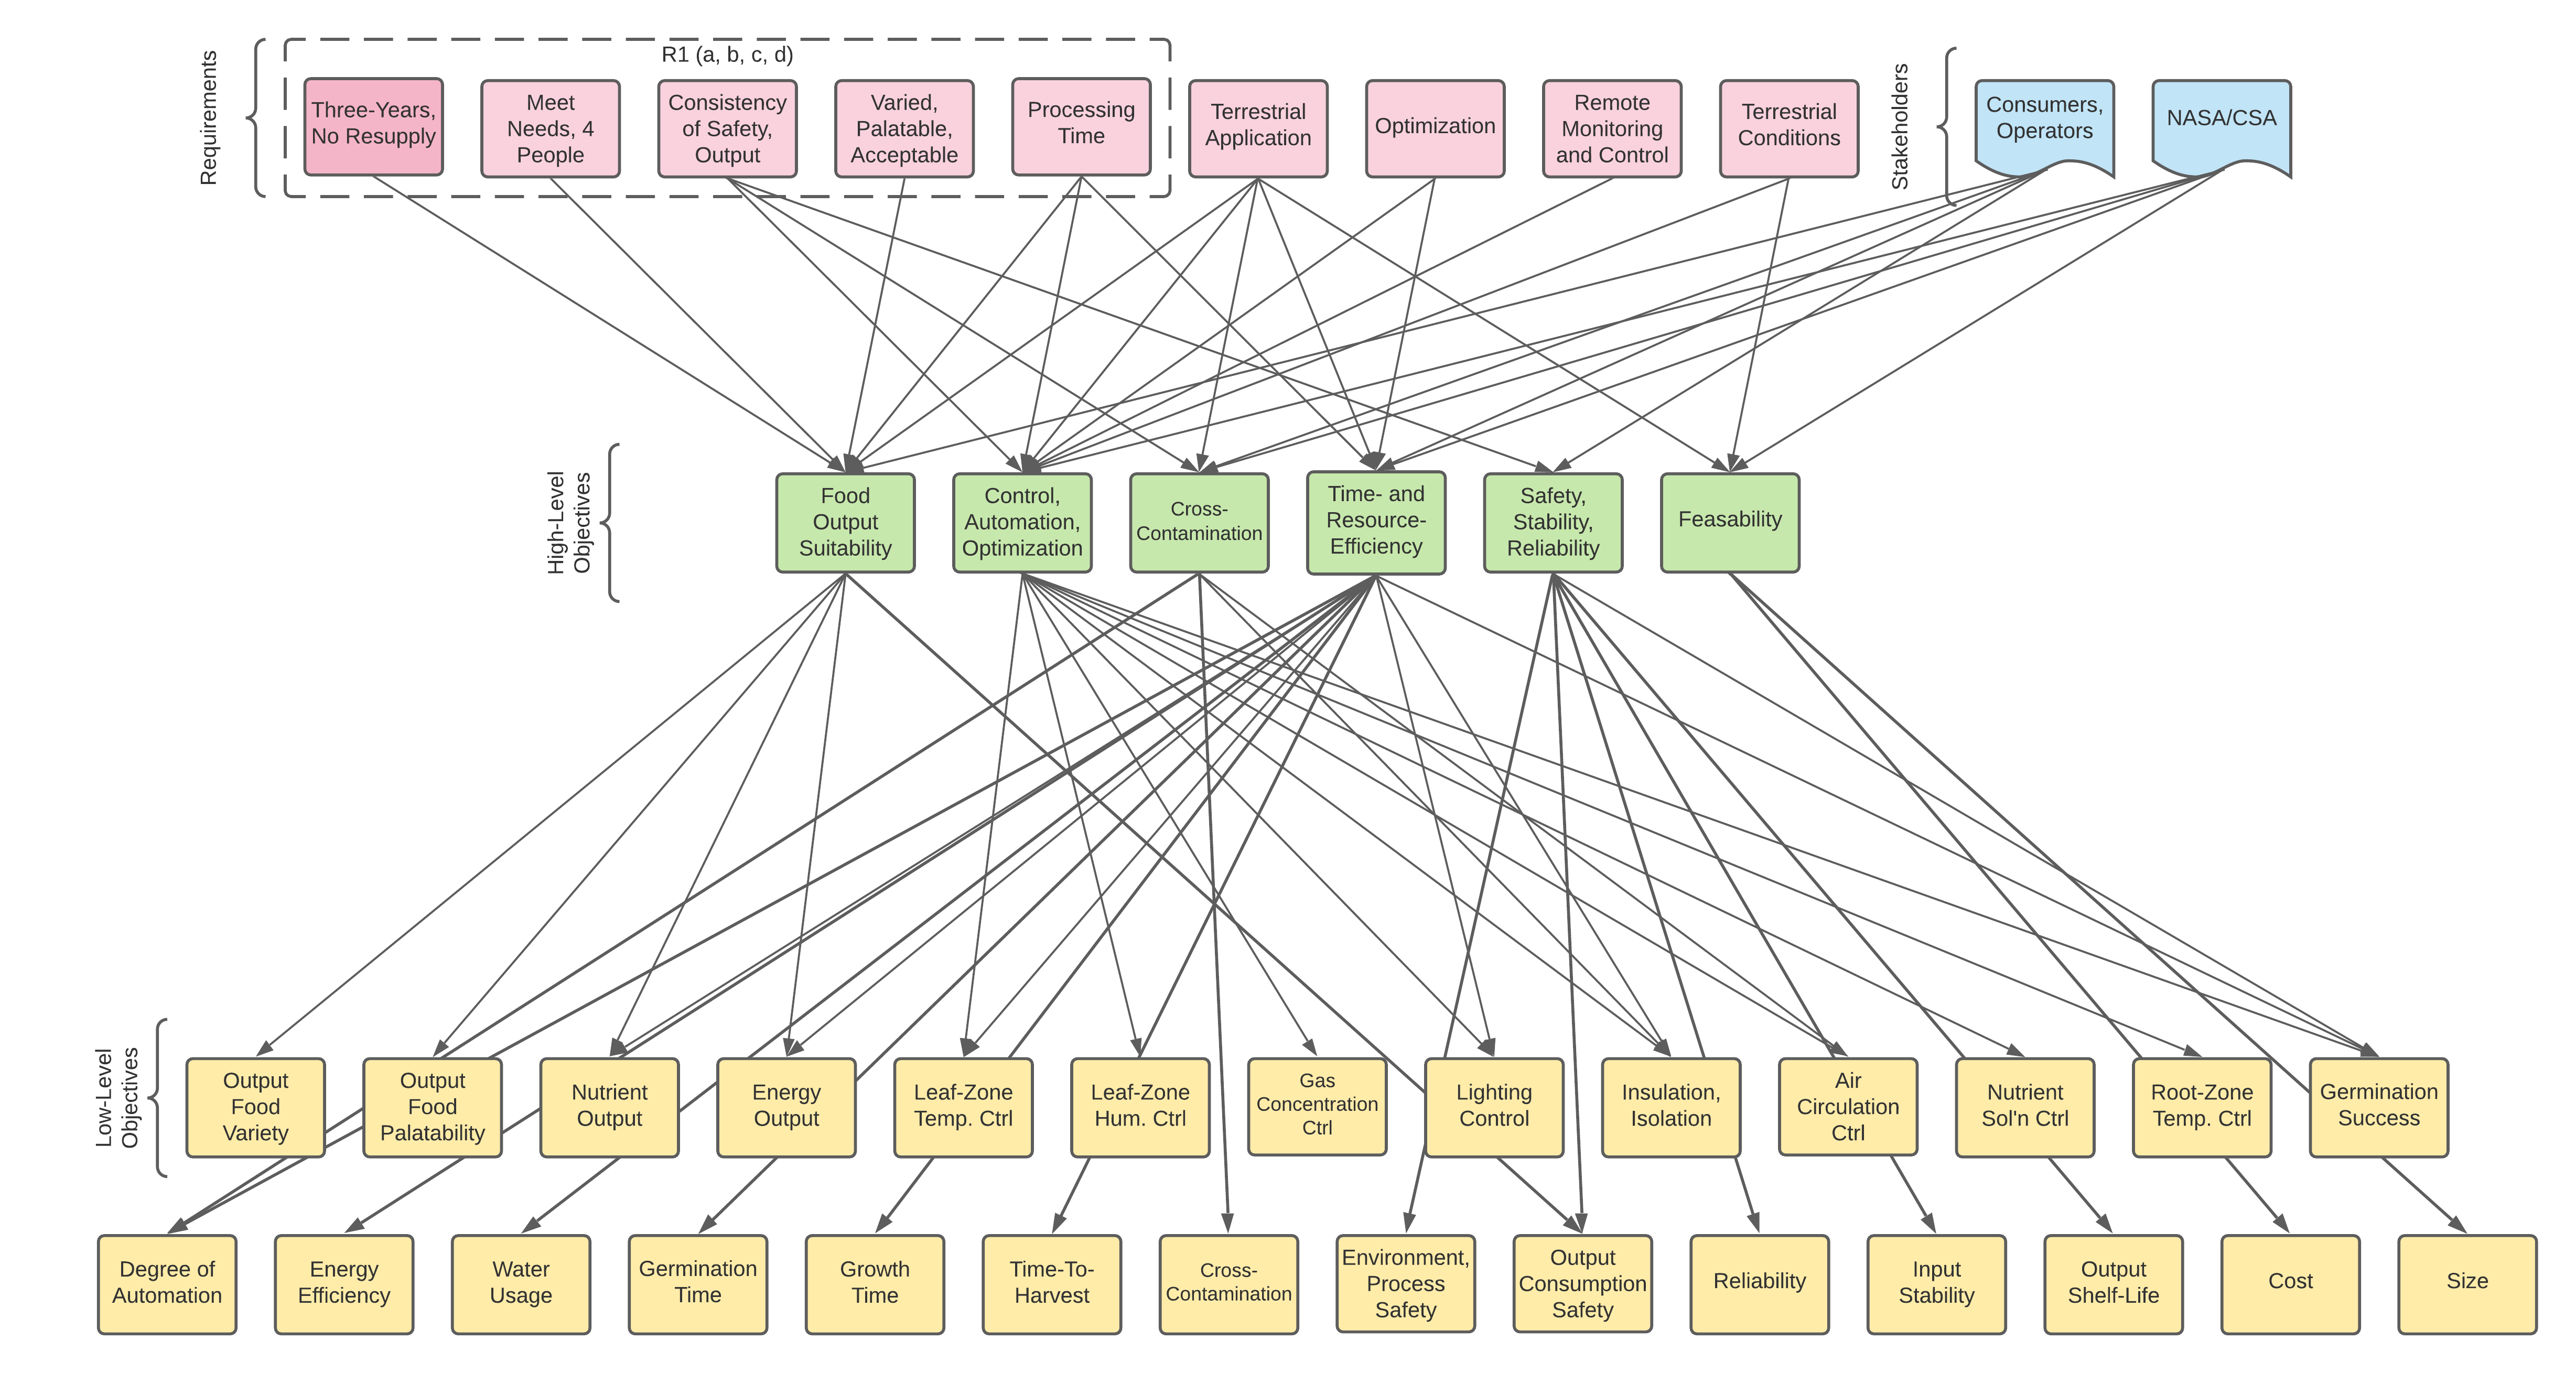
\includegraphics[width=\textwidth,angle=90,origin=c]{../assets/figures/requirements.png}
  \caption{Requirements inheritance graph.}
  \label{fig:requirements-graph}
\end{figure}

\end{appendices}

\clearpage

% References
\bibliographystyle{IEEEtran}
\bibliography{references}

\end{document}